\documentclass[12pt,a4paper]{article}
\usepackage[marginparsep=8pt,left=2.5cm,right=2.5cm,top=2.5cm,bottom=3cm]{geometry}
\usepackage[T1]{fontenc}
\usepackage[utf8]{inputenc}
\usepackage{graphicx}

\usepackage[labelformat=empty]{caption}

\usepackage{hyperref}
\hypersetup{
    colorlinks=true,
    linkcolor=blue,
    filecolor=magenta,
    urlcolor=cyan,
}

\usepackage{fontspec}
%\setmainfont[]{./fonts/Calluna-Regular.otf}

\begin{document}
\pagenumbering{gobble}

\center{\textbf{\fontsize{25}{30}\selectfont Booleovský model}}
\center{{\fontsize{14}{30}\selectfont Daniel Honys}}

\flushleft

\section*{Popis projektu}
Cílem projektu je implementace Booleovského modelu pro získávání informací z
kolekce textových dokumentů. Model umožňuje uživateli využití booleovského
dotazu pro získání seznamu dokumentů, které daný dotaz splňují.

\section*{Způsob řešení}
Předpokládáme, že máme nějakou kolekci textových dokumentů. Před schopností
dotazování nad kolekcí je nutné jednotlivé dokumenty kolekce předzpracovat. Z
jednotlivých dokumentů jsou vyextrahovány dostatečně výrazné termy, které se v
textu dokumentu vyskytují. Takové termy v podstatě tvoří jakýsi souhrn
důležitých informací v dokumentu. Termy ze všech dokumentů pak tvoří slovník.
Každý term má vlastní list dokumentů, kde se vyskytuje, což je pak využito při
vyhodnocení dotazu.

\section*{Implementace}
Implementace projektu byla rozdělena do podprojektů a pro automatizaci
sestavování využívala \textbf{Gradle}. Vše bylo vyvíjeno v jazyce \textbf{Java}.

\subsection*{bm-scraper}
Podprojekt, který má za úkol vytvoření kolekce různých článků z Wikipedie.
Využívá odkaz, který uživatele přesměruje na random článek na Wikipedii
(\href{https://en.wikipedia.org/wiki/Wikipedia:Special:Random}{Wikipedia Special Random}).
Ze stránky článku se pak vezme několik odstavců. Pro extrakci odstavců je využita
knihovna \textbf{jsoup}. Odstavce společně s názvem a odkazem na článek jsou
uloženy do souboru. Pro každý článek je jeden soubor.

\subsection*{bm-preprocess}
Tento podprojekt se zabývá předzpracováním kolekce. Předzpracování zahrnuje
načtení souboru obsahující článek, zpracování textu a extrakce jeho termů, zde
jsem využil \textbf{CoreNLP} knihovnu od Stanfordovi univerzity. Text článku,
jeho termy a relace jsou zapsány do databáze.

\begin{flushleft}
Postup:
\end{flushleft}
\begin{enumerate}
  \item Načtení textu ze souboru
  \item Tokenizace
  \item Lemmanizace
  \item Odstranění nedůležitých znaků a slov (číslovky, speciální znaky,
  zkratky, …)
  \item Odstranění stopslov (často vyskytujících se slov)
  \item Odstranění slov pod určitou délku
  \item Filtrace unikátních slov
  \item Uložení článku, termů a relací do databáze
\end{enumerate}

\begin{figure}[h]
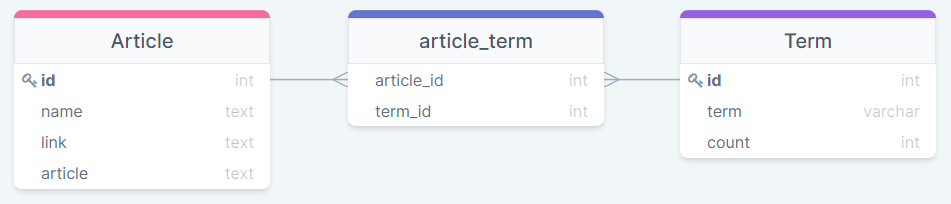
\includegraphics[width=\textwidth]{./images/database.png}
\caption{Databázové schéma}
\end{figure}

Jako relační databázi jsem zvolil \textbf{MySQL}.

\subsection*{bm-web-app}
V tomto sub projektu je realizovaná webová aplikace. Aplikace využívá
\textbf{Spring boot} jako backend framework. A frontend aplikace je realizován
pomocí \textbf{Vaadin} frameworku.

\begin{flushleft}
Uživatel zadá dotaz, který chce provést nad databází. Jako první dojde ke
kontrole, zda dotaz splňuje pravidla definované gramatiky. Pro tuto kontrolu
jsem využil knihovny \textbf{ANTLR v4} (v ní si člověk definuje pravidla
gramatiky a knihovna pak kontroluje správnost dotazu). Pokud je dotaz v
pořádku, tak je proveden nad databází a výsledek je pak vyobrazen uživateli.
Pokud je dotazem něco v nepořádku, je uživateli zobrazena error zpráva.
\end{flushleft}

\begin{flushleft}
Aplikace dále umožnuje uživateli si prohlédnou jednotlivé termy a články, které
se v databázi nacházejí.
\end{flushleft}

\begin{flushleft}
Webová aplikace společně s databází jsou pak hostované za pomoci
\textbf{Dockeru} ve VPS.
\end{flushleft}

\section*{Příklad výstupu}

\begin{center}
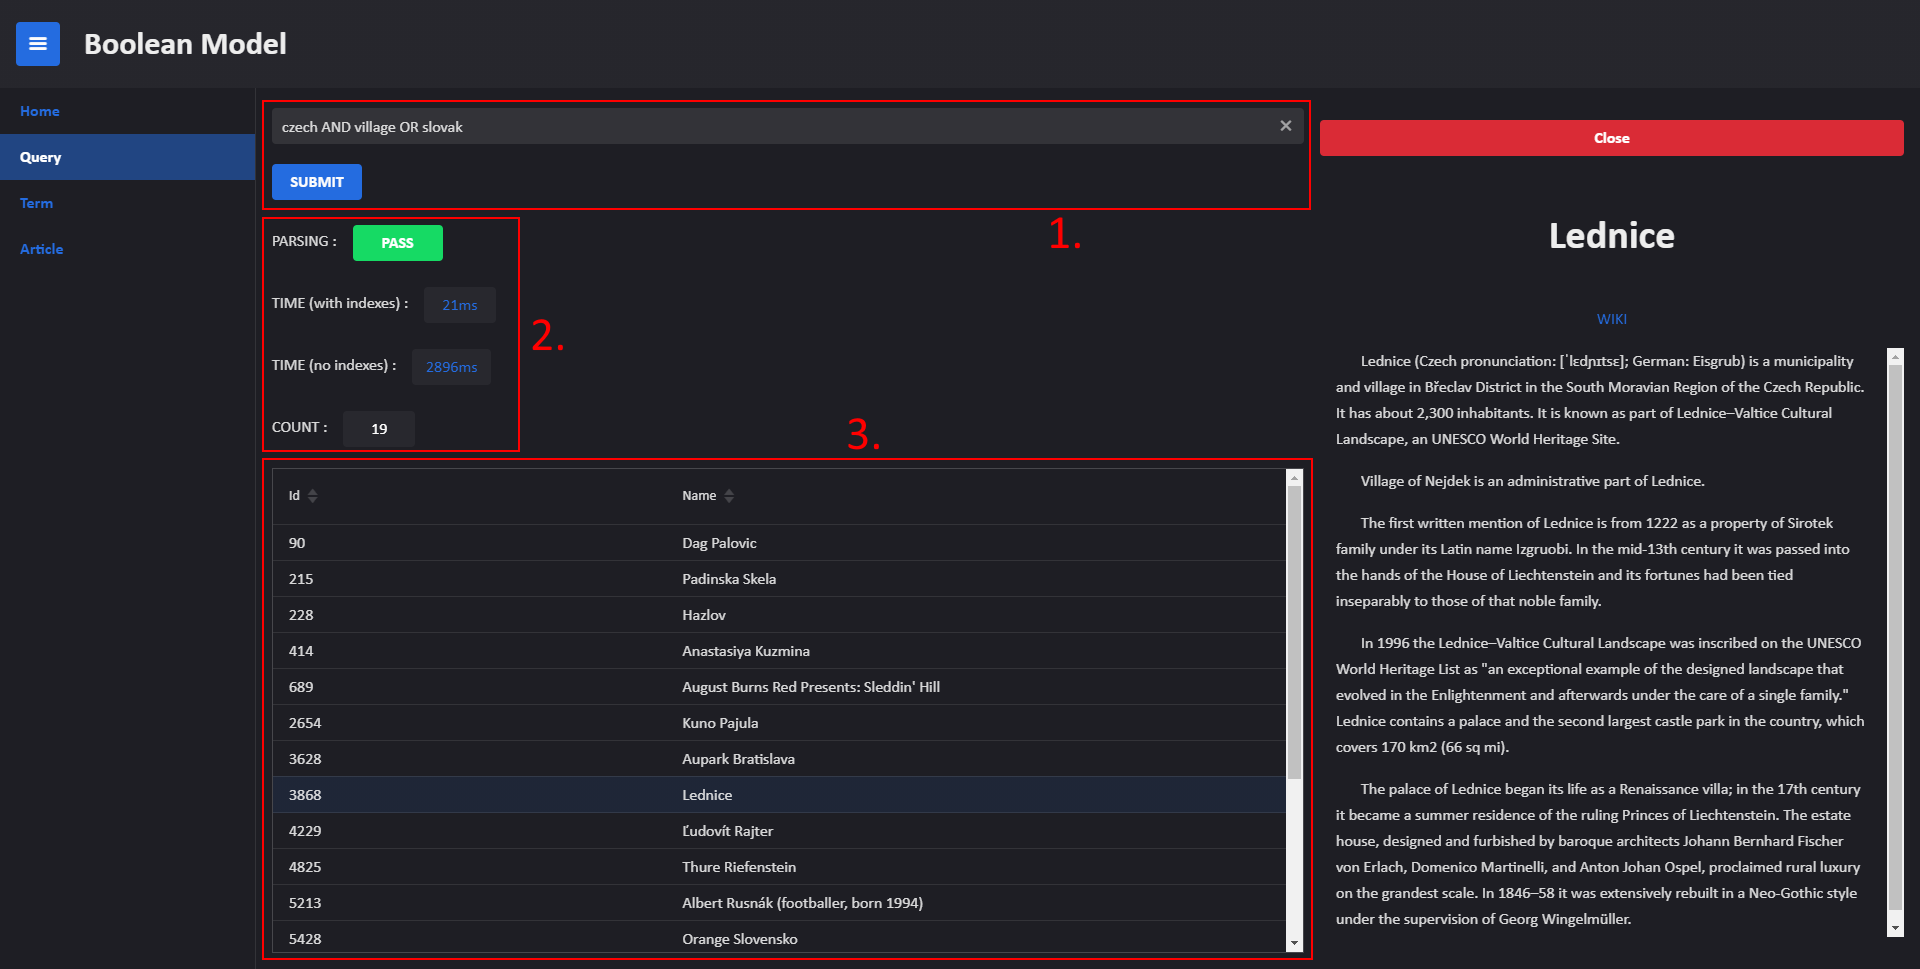
\includegraphics[width=\textwidth]{./images/result.png}
\end{center}
Na obrázku je vidět vyhodnocení dotazu „czech AND village OR slovak“.

\begin{enumerate}
  \item Místo pro zadání dotazu
  \item Informace o vyhodnocení dotazu
  \item Seznam dokumentů, které splňují dotaz
\end{enumerate}

Při selekci nějakého článku je uživateli otevřen náhled článku, kde se nachází
i odkaz na původní stránku Wikipedie, kde se článek nachází.

\section*{Experimentální sekce}
V této sekci bych se chtěl podívat na rychlost vyhodnocení dotazu.

\begin{center}
  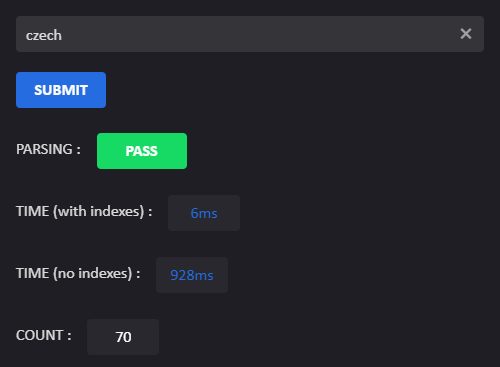
\includegraphics[width=.45\textwidth]{./images/short.png}
  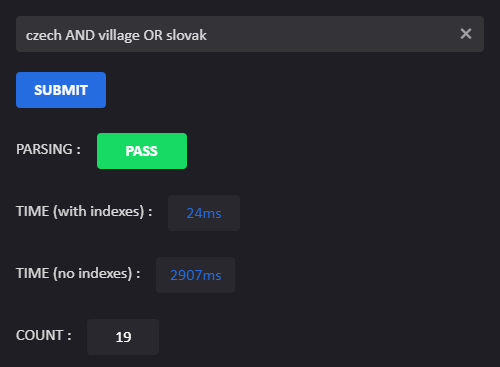
\includegraphics[width=.45\textwidth]{./images/long.png}
\end{center}

Zde můžeme vidět dva různě komplexní dotazy. Vidíme, že komplexnější dotaz trval
na vyhodnocení déle a tím pádem můžeme říct, že rychlost vyhodnocení je přímo
závislá na komplexitě dotazu.

\begin{flushleft}
Při porovnání času s indexem a bez, je vidět že bez použití indexu je
vyhodnocení značně pomalejší. Index jako takový je datová struktura, která
pomáhá databázovému stroji urychlit procházení tabulky nad kterou je zrovna
prováděný dotaz. Bez jeho využití je databázový stroj nucen projít veškeré
záznamy v tabulce sekvenčně, proto je čas bez využití indexu o tolik větší.
\end{flushleft}

\section*{Diskuse}
V projektu je prostor pro přidání pár funkcionalit a optimalizací (např.: u
dokumentu ukazovat seznam termů, které se v něm vyskytují; optimalice
booleovského dotazu přezávorkováním podle počtu dokumentů ve kterých se term
vyskytuje, …) ale myslím si, že moje řešení je celkem obstojným „proof of
concept“.

\section*{Závěr}
Boolean model se ukázal jako dobrý způsob vyhledávání za předpokladu, že přesně
víme, co hledáme. Jeho nevýhodou však je že nebere v potaz žádný ranking či jiné
relace mezi dokumenty.

\end{document}
